\documentclass[11pt, fontset=windows, ignorenonframetext]{beamer}  % ignorenonframetext 忽略任何 frame 之外的所有文本

\usepackage[noindent]{ctex} % 中文
\usepackage[T1]{fontenc} %  风格数学字体
\usepackage{hyperref} % 超链接命令
\usepackage{graphicx} % 支持插图
\usepackage{subfigure} % 子图片
\usepackage{times} % 使用 Times New Roman 字体
\usepackage{pgf,tikz} % 在 tex 系统中使用 pgf 绘图
\usepackage{bookmark}
\usepackage{booktabs} % 三线表
\usepackage{latexsym} % 数学符号环境
\usepackage{amsmath,amsfonts,amssymb,amscd,amsthm,calligra,mathrsfs}
\usepackage{xcolor,comment,pstricks,listings,stackengine}
\usepackage{multicol,multirow} % 多栏
\usepackage{array} % 表格
\usepackage{ragged2e} % 段落对齐
\usepackage[english]{babel}
\usepackage{rotating} % 可以将文本、表格、图形旋转
\usepackage{enumerate} % 列表环境
\usepackage{bm} % 提供将数学符号加粗的命令 \bm
\usepackage{csquotes} % 引号
\usepackage{fontspec} % 设置字体


%---------- START PREAMBLE ----------

%-------- theme --------
\usetheme{Madrid}
\useoutertheme[subsection=false]{smoothbars} % 把 Navigation dots 放在一行

\makeatletter
\AtBeginDocument{
\pgfdeclareverticalshading{beamer@barshade}{\the\paperwidth}{%
        color(0ex)=(black);%
        color(0.5ex)=(section in head/foot.bg);%
        color(4ex)=(section in head/foot.bg)%
    }
}
\makeatother

% \setbeamertemplate{blocks}[rounded][shadow=false]  % 去掉 block 的阴影
% \setbeamertemplate{title page}[default][colsep=-4bp,rounded=true]  % 去掉标题框的阴影
\setbeamertemplate{frametitle}[default][colsep=-4bp,rounded=false,shadow=false]  % 去掉每个 frame 的 标题框的阴影

%-------- color --------
\definecolor{CufeBlue}{RGB}{45,122,200}  % also recommend 34,92,150
\definecolor{DeepCufeBlue}{RGB}{23,61,100}
\usecolortheme[named=CufeBlue]{structure}  % 主体颜色
\setbeamercolor{section in head/foot}{fg=white,bg=DeepCufeBlue}  % 顶/底部导航栏颜色
\setbeamercolor{subsection in toc}{fg=CufeBlue} % 目录中子标题的文字颜色

\def\cmd#1{\texttt{\color{red}\footnotesize $\backslash$#1}} % 红字 -> 标识“命令”
\def\env#1{\texttt{\color{blue}\footnotesize #1}} % 蓝字 -> 标识“环境”

%-------- set color of 'example block' to crimson theme --------
\definecolor{examplegold}{RGB}{180,147,85}
\definecolor{lightgray}{gray}{0.96}  % 数值越大,颜色越浅
\setbeamercolor{block body example}{bg=lightgray}
\setbeamercolor{block title example}{fg=white, bg=examplegold}

%-------- font --------
% %  定义字体
% \newfontfamily\tnr{Times New Roman}
% \setbeamerfont{structure}{family=\tnr,series=\bfseries}
% \setbeamerfont{normal text}{family=\sffamily,series=\mdseries}
% \setbeamerfont{alerted text}{family=\sffamily,series=\bfseries}
% \setbeamerfont{frametitle}{family=\rmfamily,series=\bfseries}
\setbeamerfont{structure}{family=\rmfamily,series=\bfseries}
\setbeamerfont{subsection in toc}{family=\rmfamily, size=\large}  % 目录中标题的字体及大小
\setbeamerfont{subsection in toc}{family=\rmfamily, size=\normalsize}  % 目录中子标题的字体及大小
\usefonttheme[stillsansseriftext]{structurebold}
\setbeamerfont{section in head/foot}{size=\tiny}  % 设置顶部和底部导航栏的字体大小

%-------- highlight the title of the current section --------
\AtBeginSection[]
{
\begin{frame}
    \frametitle{Presentation Outline}
    \tableofcontents[currentsection]
\end{frame}
}

%-------- misc structure --------
\useoutertheme[footline=authortitle,subsection=false]{miniframes}
\useinnertheme{rounded} % 设置 block 为圆角(默认增加阴影)
\addtobeamertemplate{block begin}{}{\justifying}
% \newtheorem{remark}[theorem]{Remark}

% ======== 自定义中文环境名称 =========
\newtheorem{Cexample}{例} % 整体编号
\newtheorem{Calgorithm}{算法}
\newtheorem{Ctheorem}{定理}[section] % 按 section 编号
\newtheorem{Cdefinition}[theorem]{定义}
\newtheorem{Caxiom}[theorem]{公理}
\newtheorem{Cproperty}[theorem]{性质}
\newtheorem{Cproposition}[theorem]{命题}
\newtheorem{Clemma}[theorem]{引理}
\newtheorem{Ccorollary}[theorem]{推论}
\newtheorem{Cremark}[theorem]{注解}
\newtheorem{Ccondition}[theorem]{条件}
\newtheorem{Cconclusion}[theorem]{结论}
\newtheorem{Cassumption}[theorem]{假设}
% 编号精确到 subsection
\numberwithin{subsection}{section}
\numberwithin{theorem}{subsection}

% \setlength{\parindent}{1.5em} % 首行缩进
\setlength{\parskip}{0.5em} % 段落间距
\renewcommand{\baselinestretch}{1.1} % 1.2倍默认行间距
% \linespread{1} % 单倍 word 行间距
\renewcommand{\indent}{\hspace*{2em}} % 定义单次缩进距离
\setbeamertemplate{definitions}[numbered] % 定义环境显示编号
\setbeamertemplate{theorems}[numbered] % 定理标题显示编号
\setbeamertemplate{caption}[numbered] % 图和表格的标题显示标号

\usepackage[justification=centering]{caption} % 控制浮动体标题的格式
\renewcommand{\qedsymbol}{$\blacksquare$}

% \setenumerate[1]{itemsep=0pt,partopsep=0pt,parsep=\parskip,topsep=5pt}
% \setitemize[1]{itemsep=0pt,partopsep=0pt,parsep=\parskip,topsep=5pt}
% \setdescription{itemsep=0pt,partopsep=0pt,parsep=\parskip,topsep=5pt}

%-------- for bibliography -----------------
\usepackage[backend=bibtex,bibstyle=authoryear,citestyle=authoryear,sorting=nyt,natbib=true]{biblatex}
\setbeamertemplate{bibliography item}{}  % 参阅:https://tex.stackexchange.com/questions/585635/beamer-biblatex-authoryear-causes-problem-with-insertbiblabel
\addbibresource{./Reference/RefTemplate.bib}
\setbeamertemplate{frametitle continuation}{\frametitle{\color{white}List of References}}

%-------- Backgound -------------------
\usebackgroundtemplate{%
	\tikz[overlay,remember picture] \node[opacity=0.03, at=(current page.center)] {
		
\includegraphics[height=4.6in,width=4.6in]{./Figure/CUFE_logo.jpg}};
}

%---------- PREAMBLE END ----------


%--------- START EDITING HERE ---------------------
\title[One Example for Academic Slides]{One Example for Academic Slides}
% \subtitle{A Study of Actor ARATA's Work}

\author [Arata Iura]{\textbf{Shuuji Murakumo, Kei Nakado, Kenichirou Kase}}
\institute[Central University of Finance and Economics] { \emph{Presenter:} \textbf{Arata Iura (B. A. Japanese Literature)}\\[1em]
	Department of Japanese\\School of Foreign Studies\\Central University of Finance and Economics\\[1em]

\includegraphics[scale=0.1]{./Figure/CUFE_logo.png}}

\date[April 21, 2022]{\footnotesize Online Seminar - \textbf{April 21, 2022}}

%--------- START DOCUMENT ------------------
\begin{document}

\begin{frame}{\titlepage}\end{frame}

\begin{frame}{\frametitle{Presentation Outline}\tableofcontents[sectionstyle=show,subsectionstyle=hide,subsubsectionstyle=hide]}\end{frame}

%--------- INTRODUCTION ----------------------
\section{Introduction}

\begin{frame}
	\frametitle{Introduction}
		\justifying % 两端对齐
		Lorem ipsum dolor sit amet, consectetur adipiscing elit. Duis ut imperdiet lorem. Sed imperdiet sit amet quam sit amet molestie. Curabitur elementum magna sem, eu viverra augue pharetra quis. Phasellus ut turpis vel nunc fermentum ornare. Maecenas sit amet semper leo. Praesent sodales vel lectus sed hendrerit.
\end{frame}

%---------- DEFINITION/PRELIMINARY ---------------------
\section{Working Definitions}

\subsection{WD1}
\begin{frame}
	\frametitle{WD1}
	\begin{Cdefinition}\label{def1} A  set $M \subseteq E(G)$ is an \emph{edge dominating set of $G$} if every $u \in E(G) \backslash M$ is adjacent to some $v \in M$. The \emph{edge domination number of $G$}, denoted by $\gamma_{e}(G)$, is the minimum cardinality of an edge dominating set of $G$. Any edge dominating set of $G$ with cardinality $\gamma_{e}(G)$ is referred to as a \emph{$\gamma_{e}$-set of $G$}.
	\end{Cdefinition}
\end{frame}

\begin{frame}
	\setlength{\parskip}{1em} % 设置 frame 里的段落间距
	\frametitle{WD1}
	column 可以用来给内容分栏。
	
	insert a sample frame with two columns
	
	\begin{columns}
		\column{0.5\textwidth}
		\begin{itemize}
			\setlength{\itemsep}{5pt}  % 设置列表各条目间距
			\item A $(t,n)$ threshold secret sharing scheme allows a dealer to split her secret $s$ into $n$ pieces (also called shares) and distribute them among $n$ parties. 
			\item In a threshold scheme any $t$ or more than $t$ shareholders can reconstruct the secret. 
		\end{itemize}
		\bigskip
		\column{0.5\textwidth}
		\begin{figure}[ht]
			\centering
			% Requires \usepackage{graphicx}
			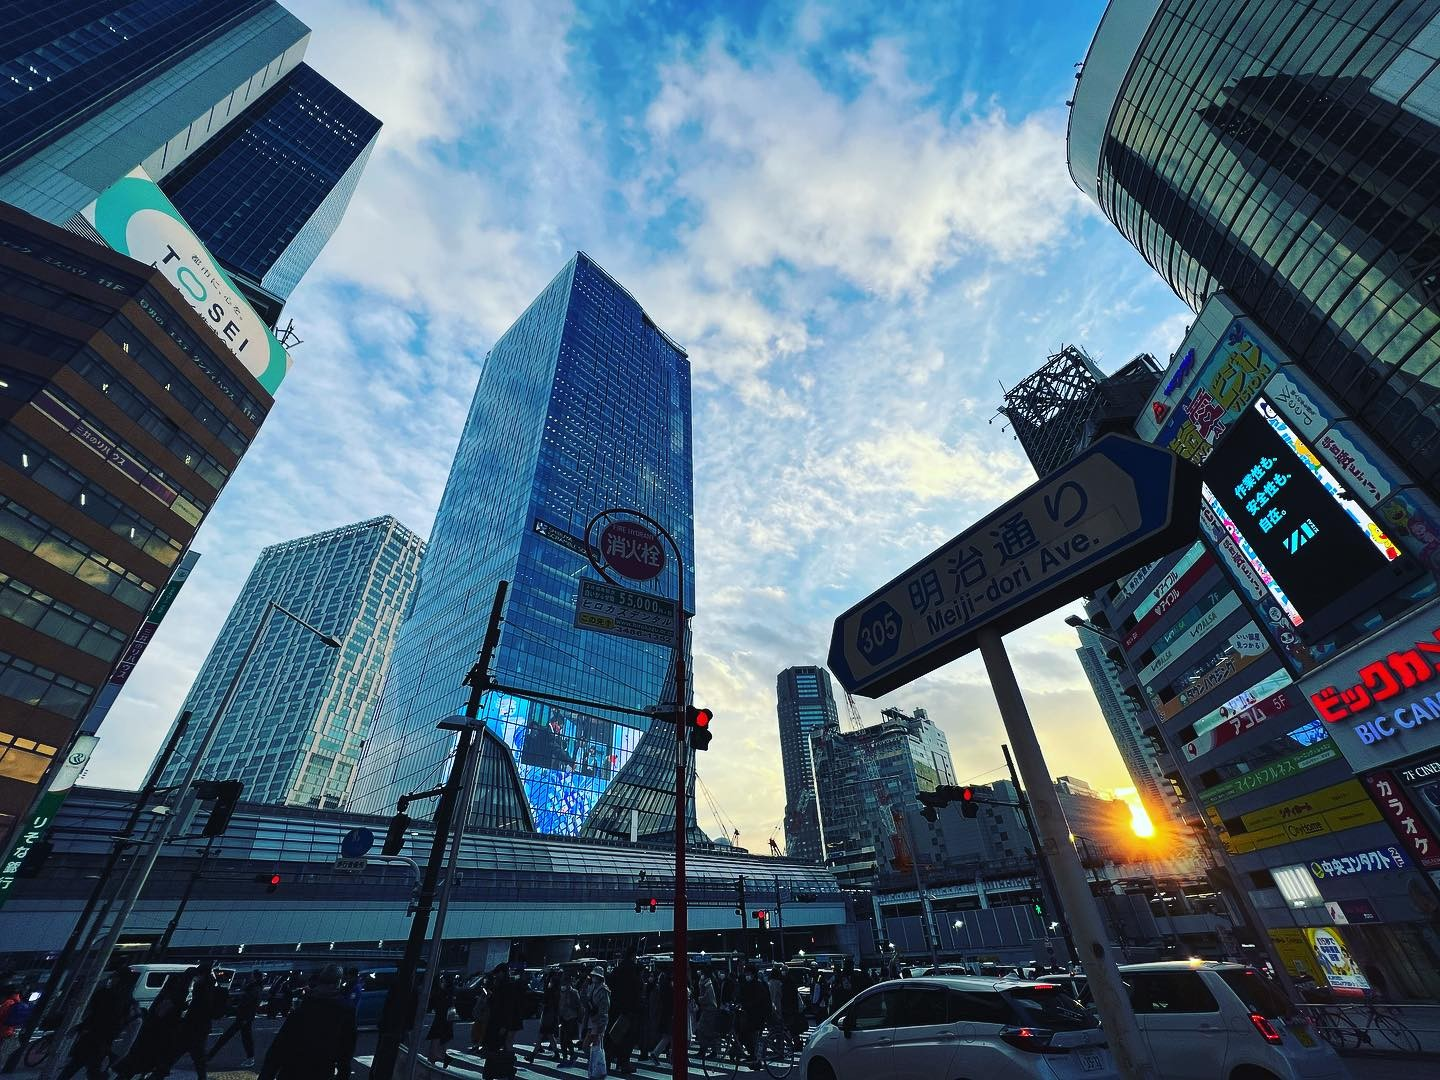
\includegraphics[width=0.7\textwidth, height=0.4\textheight]{./Figure/arata_1.jpg}
			\caption{INS@arata}
			\label{F1}
		\end{figure}
	\end{columns}
\end{frame}

\subsection{WD2}
\begin{frame}
	\frametitle{WD2}
	\begin{Cdefinition}\label{def2}
		无编号公式 % 加 * 
		\begin{equation*}
			J(\theta) = \mathbb{E}_{\pi_\theta}[G_t] = \sum_{s\in\mathcal{S}} d^\pi (s)V^\pi(s)=\sum_{s\in\mathcal{S}} d^\pi(s)\sum_{a\in\mathcal{A}}\pi_\theta(a|s)Q^\pi(s,a)
		\end{equation*}
	\end{Cdefinition}

	多行多列公式
	\footnote{如果公式中有文字出现,请用 $\backslash$mathrm\{\} 或者 $\backslash$text\{\},不然就会变成 $clip$,而不是 $\mathrm{clip}$ 。}
    % 使用 & 分隔
    \begin{align}
        Q_\mathrm{target}&=r+\gamma Q^\pi(s^\prime, \pi_\theta(s^\prime)+\epsilon)\\
        \epsilon&\sim\mathrm{clip}(\mathcal{N}(0, \sigma), -c, c)\nonumber
    \end{align}
\end{frame}

\subsection{WD3}
\begin{frame}
	\frametitle{WD3}
	\begin{block}{Remark}
		编号多行公式
        % Taken from Mathmode.tex
        \begin{multline}
            A=\lim_{n\rightarrow\infty}\Delta x\left(a^{2}+\left(a^{2}+2a\Delta x+\left(\Delta x\right)^{2}\right)\right.\label{eq:reset}\\
            +\left(a^{2}+2\cdot2a\Delta x+2^{2}\left(\Delta x\right)^{2}\right)\\
            +\left(a^{2}+2\cdot3a\Delta x+3^{2}\left(\Delta x\right)^{2}\right)\\
            +\ldots\\
            \left.+\left(a^{2}+2\cdot(n-1)a\Delta x+(n-1)^{2}\left(\Delta x\right)^{2}\right)\right)\\
            =\frac{1}{3}\left(b^{3}-a^{3}\right)
        \end{multline}
	\end{block}
\end{frame}

\begin{frame}
	\frametitle{WD3 (Cont.)}
	\justifying % 两端对齐
	Lorem ipsum dolor sit amet, consectetuer adipiscing elit.

	\begin{Ctheorem}
		\justifying % 两端对齐
		Lorem ipsum dolor sit amet, consectetuer adipiscing elit. Ut purus elit, vestibulum ut, placerat ac, adipiscing vitae, felis. Curabitur dictum gravida mauris. Nam arcu libero, nonummy eget, consectetuer id, vulputate a, magna.
	\end{Ctheorem}

	\begin{table}[h]
        \centering
        \begin{tabular}{c|c}
            Microsoft\textsuperscript{\textregistered}  Word & \LaTeX \\
            \hline
            文字处理工具 & 专业排版软件 \\
            公式排版差强人意 & 尤其擅长公式排版 \\
            二进制格式,兼容性差 & 文本文件,易读、稳定 \\
        \end{tabular}
    \end{table}

\end{frame}

\begin{frame}
	\frametitle{WD3 (Cont.)}
	\justifying % 两端对齐
	Lorem ipsum dolor sit amet, consectetuer adipiscing elit.

	\begin{alertblock}{Important theorem}
		\justifying % 两端对齐
		Lorem ipsum dolor sit amet, consectetuer adipiscing elit. Ut purus elit, vestibulum ut, placerat ac, adipiscing vitae, felis. Curabitur dictum gravida mauris. Nam arcu libero, nonummy eget, consectetuer id, vulputate a, magna.
	\end{alertblock}

	\begin{enumerate}
		\item English
		\item Chinese
		\begin{itemize}
			\item[Ex1] 中文 1
			\item[Ex2] 中文 2
		\end{itemize}
	\end{enumerate}

\end{frame}

\begin{frame}
	\frametitle{WD3 (Cont.)}
	\begin{Cexample}
	\justifying
		\normalfont{The sets $M_{1}=\{a, c, f\}, M_{2}=\{d, h\}$, and $M_{3}=\{a, e, g, h\}$ are edge dominating sets of $G$ in Figure 1.5. Moreover, $M_{2}=\{d, h\}$ is a minimum edge dominating set of $G$. Thus, $\gamma_{e}(G)=\left|M_{2}\right|=2$.}
		\begin{figure}[ht]
			\centering
			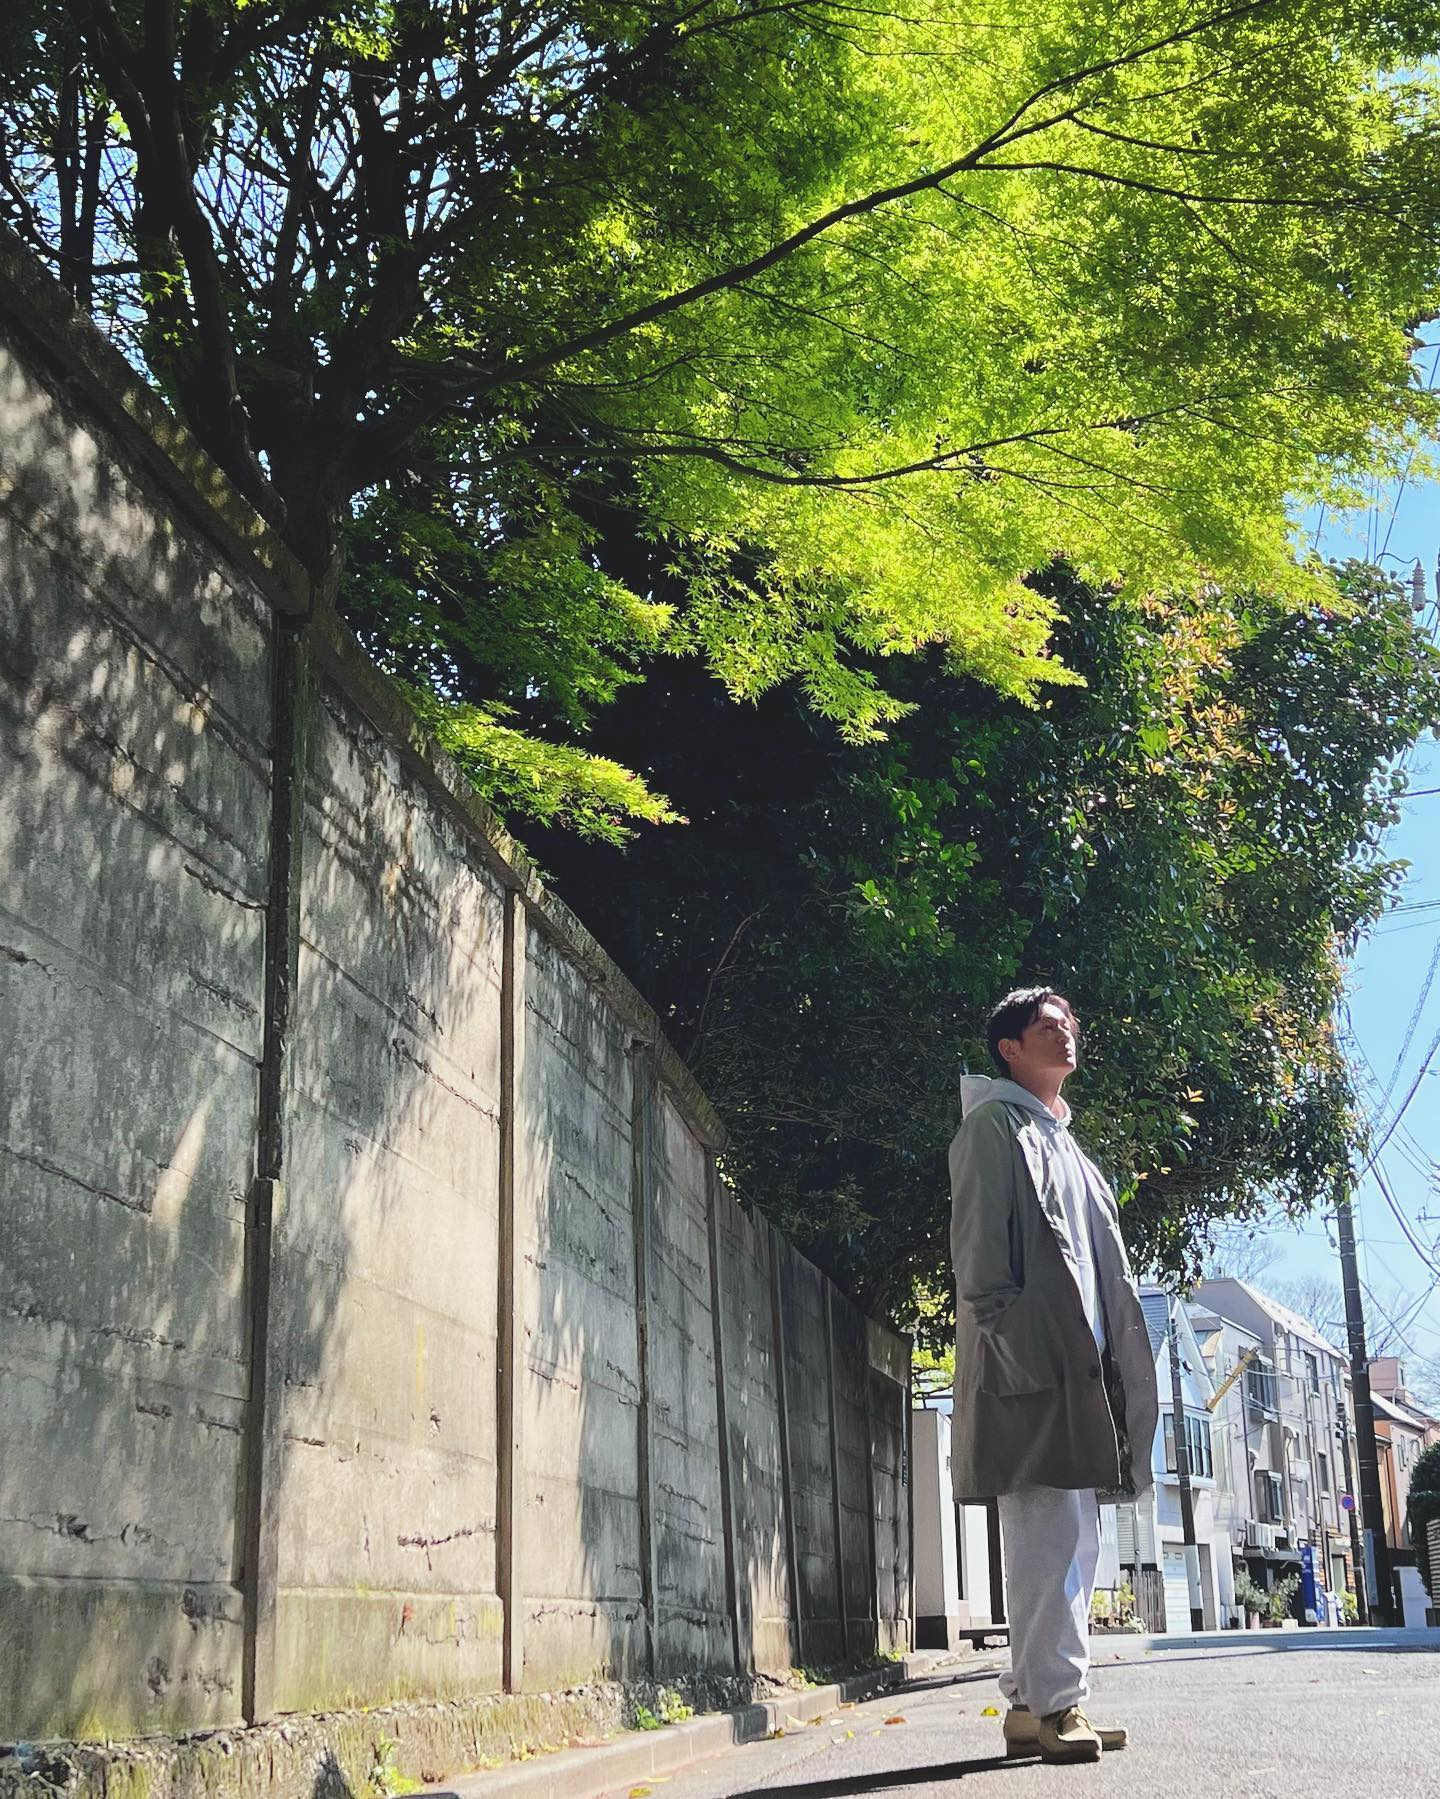
\includegraphics[width=0.2\textwidth, height=0.3\textheight]{./Figure/arata_2.jpg}
			\captionsetup{justification=centering}
			\caption{A graph $G$ with $\gamma_{e}(G)=2$.\label{edom}}
		\end{figure}
	\end{Cexample}
\end{frame}

%----------- MAIN RESULTS ------------------------------
\section{Results}

	\begin{frame}{Results}
		\begin{Cremark}\label{rem2}
			A set $S$ is an outer-connected edge dominating set of a graph $G$ if $S$ is an edge dominating set such that $H_{E(G) \backslash \mathrm{S}}$ does not have component isomorphic to $K_{2}$ or $S=E(G)$.
		\end{Cremark}
		\pause
		\indent To see this, consider graphs $G_{1}=P_{3}, G_{2}=P_{4}$, and $G_{3}=C_{8}$ in Figure \ref{F2}.
		Then, $\gamma_{oce}(P_{3})=2, \gamma_{oce}(P_{4})=3$, and $\gamma_{o c e}(C_{8})=4$.
	\end{frame}

	\begin{frame}{Results (Cont.)}
		\begin{exampleblock}{命令}
			\centering
			\footnotesize
			\begin{tabular}{llll}
				\cmd{chapter} & \cmd{section} & \cmd{subsection} & \cmd{paragraph} \\
				章 & 节 & 小节 & 带题头段落 \\\hline
				\cmd{centering} & \cmd{emph} & \cmd{verb} & \cmd{url} \\
				居中对齐 & 强调 & 原样输出 & 超链接 \\\hline
				\cmd{footnote} & \cmd{item} & \cmd{caption} & \cmd{includegraphics} \\
				脚注 & 列表条目 & 标题 & 插入图片 \\\hline
				\cmd{label} & \cmd{cite} & \cmd{ref} \\
				标号 & 引用参考文献 & 引用图表公式等\\\hline
			\end{tabular}
		\end{exampleblock}

		\begin{exampleblock}{环境}
			\centering
			\footnotesize
			\begin{tabular}{lll}
				\env{table} & \env{figure} & \env{equation}\\
				表格 & 图片 & 公式 \\\hline
				\env{itemize} & \env{enumerate} & \env{description}\\
				无编号列表 & 编号列表 & 描述 \\\hline
			\end{tabular}
		\end{exampleblock}
	\end{frame}

	\begin{frame}{Results (Cont.)}
		\begin{figure}[ht]
		\centering
		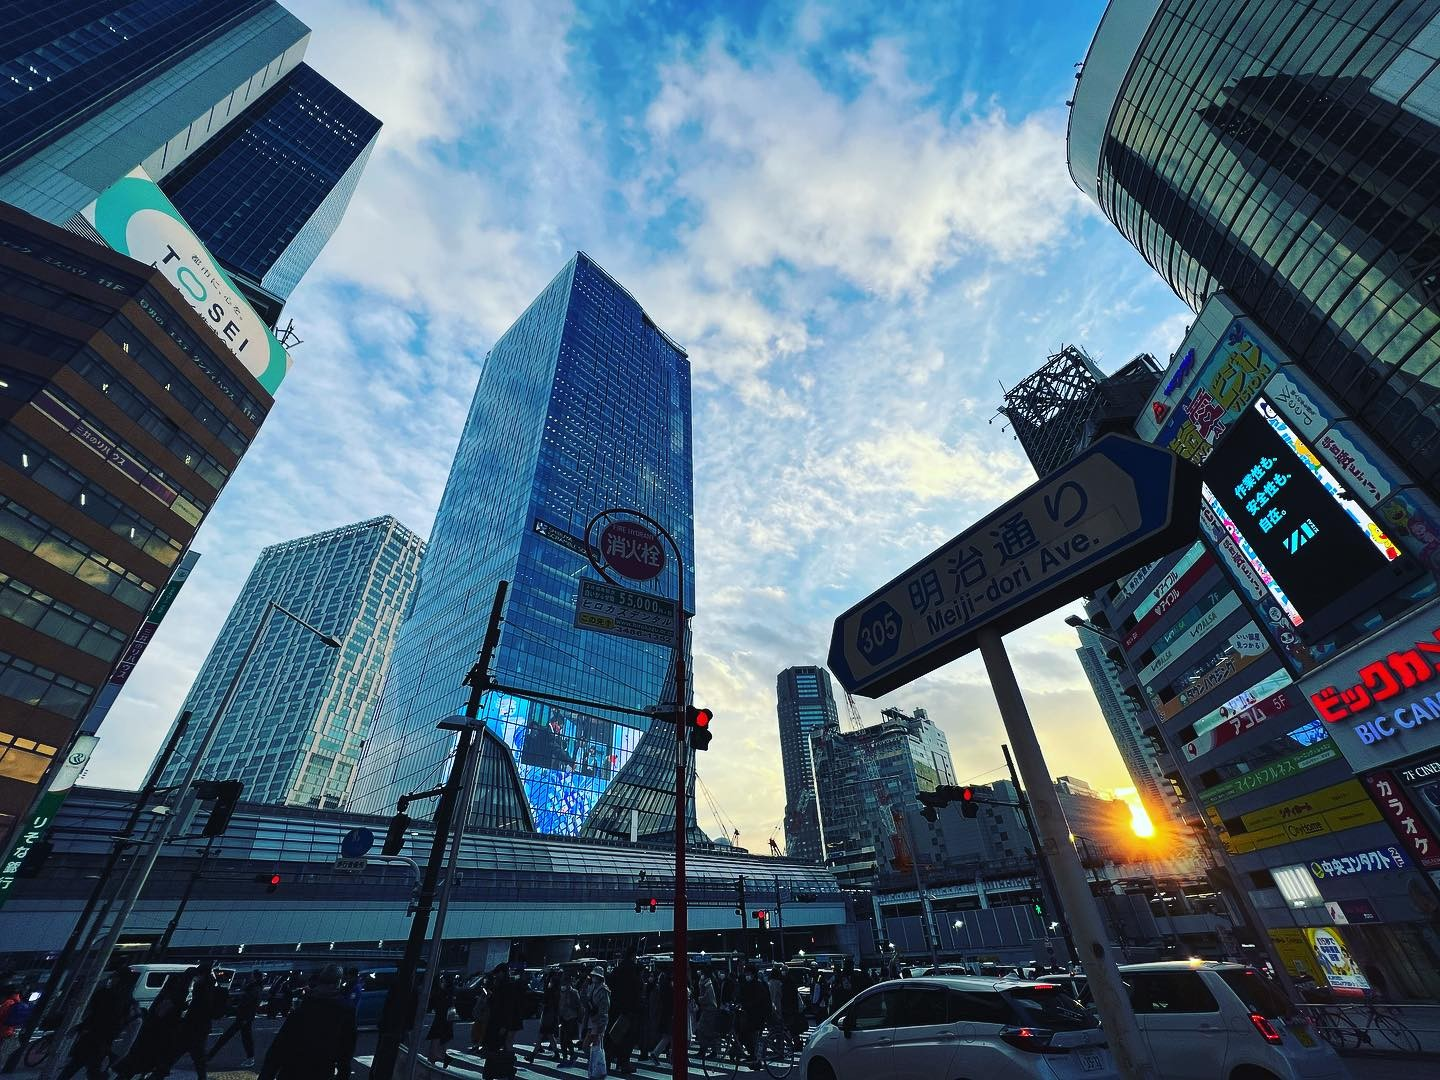
\includegraphics[width=0.4\textwidth, height=0.6\textheight]{./Figure/arata_1.jpg}
		\caption{Graphs with $\gamma_{oce}(P_{3})=2, \gamma_{oce}(P_{4})=3$, and $\gamma_{oce}(C_{8})=4$.\label{F2}}
		\end{figure} 
	\end{frame}

%---------- RECOMMENDATIONS -----------------------------
\section{Recommendations}
	\begin{frame}
		\frametitle{Recommendations}
		\justifying
		The following problems are suggested for further study:
		\footfullcite{velickovic2017graph}

		\citet{velickovic2017graph} lorem ipsum dolor sit amet, consectetur adipiscing elit. Duis ut imperdiet lorem. Sed imperdiet sit amet quam sit amet molestie. 
		
		Curabitur elementum magna sem, eu viverra augue pharetra quis. Phasellus ut turpis vel nunc fermentum ornare. Maecenas sit amet semper leo. Praesent sodales vel lectus sed hendrerit.
		\citep{kosaraju2019social,velickovic2017graph}
	\end{frame}

%----------- REFERENCES  -------------
%----------- No editing in references section ----------
%----------- edit only in 'RefTemplate.bib' ----------
	\begin{frame}[allowframebreaks]
		\justifying
		\frametitle{List of References}
		\printbibliography
	\end{frame}

%--------- THANK YOU Text --------------------------
	\begin{frame}
		\centering
		\begin{block}
			\scshape
				\begin{center}
					\Huge\emph{Thank You So Much!}
				\end{center}
		\end{block}
	\end{frame}
%----------------------------------------------------

\end{document}